\section{Spécifications}
	%@author : T'es pas à la maison mon gars , parle bien !
	%Le "aka so mega casse-couilles" etait une demande de mon voisin, je suis pas responsable :D En bref, un oubli.

\subsection{Données}
	Pour ce projet, nous avons à notre disposition une modélisation 3D de l'appartement tremplin. Cette modélisation, fournie par Kerpape, est au format .max. L'un de notre premier travail sera donc d'ouvrir ce fichier, et de le convertir au format natif d'Unity. Unity dispose bien sur de fonctionnalités d'import dans d'autres formats, mais Unity est connu pour être un peu capricieux dans ses interactions avec les .max.

	Les textures sont parfois mal gérées ou absentes, il faudra donc trouver un moyen d'interfacer correctement et efficacement la ressource avec Unity, soit avec une conversion de format de fichier, soit en réintégrant dans Unity ce qui aura été perdu à l'import.

\subsection{Logiciels}
	Au cours de ce projet, nous allons devoir travailler avec plusieurs environnements logiciels : les modeleurs 3D et les environnements de développement. La première catégorie de logiciels permet de modifier le modèle ou de créer de nouveaux éléments, comme un téléphone ; tandis que la seconde permet d'écrire la logique pour réaliser la partie interactive du projet.

	Voici les solutions logicielles que nous allons utiliser pour la réalisation :
	\subsubsection{3DSmax}
		\noindent\begin{minipage}{0.3\textwidth}
			
\includegraphics[width=\linewidth]{1-PreEtude/img/3dsmax_logo}
			\end{minipage}
			\hfill
			\begin{minipage}{0.65\textwidth}
			3DSmax\cite{3dsmax}, le célèbre modeleur 3D d'Autodesk n'est plus à présenter; aujourd'hui encore considéré comme la référence en matière de modélsation 3D, et ce depuis plus de 10 ans, il est grandement utilisé dans l'industrie vidéoludique et filmographique.
			Ce logiciel est l'évolution de 3D studio, sorti sous DOS en 1990. 3DSmax lui a succédé en 1996 et dispose de nouvelles versions stables tout les 6 mois, la dernière étant la 2015 SP2 sortie le 20 mars 2014.
			Ce logiciel est cependant vendu à un prix élevé et n'est disponible que sur Windows, ce pourquoi nous utiliserons d'autres logiciels en parallèle.
		\end{minipage}


	\subsubsection{Blender}
		\noindent\begin{minipage}{0.3\textwidth}
			
\includegraphics[width=\linewidth]{1-PreEtude/img/blender_logo}
			\end{minipage}
			\hfill
			\begin{minipage}{0.65\textwidth}
			Blender\cite{blender} est le modeleur 3D libre le plus avancé. Le projet Blender fut lancé en 1995 et était initialement un logiciel propriétaire developpé en interne par Neo Geo et Not a Number Technologies.
			Son code source fut ouvert au public le 17 septembre 2002 après une campagne de dons. Aujourd'hui distribué sous licence GNU/GPLv2, il est soutenue par la Blender Foundation. Celle ci a réalisé quelques films d'animations tels que Big Buck Bunny ou Sintel pour promouvoir le logiciel.
			Le projet est régulièrement mis à jour, la dernière version (2.72) à l'heure actuelle datant du 14 octobre 2014.
			Blender est disponible sous Windows, Mac, Linux et BSD et inclut toutes les fonctionnalités classiques d'un logiciel de se type, mais inclu aussi des fonctionnalités d'extension via des scripts Python ainsi qu'un moteur de jeu.
			Ces possibilités supplémentaires ne seront cependant pas utilisés dans ce projet, car elles ne répondent que partiellement à notre problématique.
		\end{minipage}


	\subsubsection{Unity}
		\noindent\begin{minipage}{0.3\textwidth}
			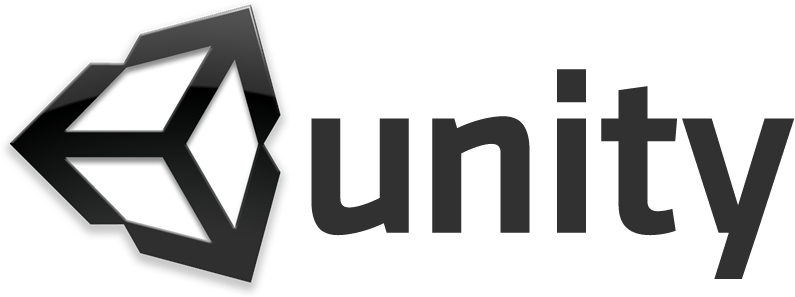
\includegraphics[width=\linewidth]{1-PreEtude/img/unity_logo}
			\end{minipage}
			\hfill
			\begin{minipage}{0.65\textwidth}
			Unity\cite{unity} est un environnement et un moteur de rendu 3D ; initialement pensé pour les jeux vidéos, il permet de créer ou modifier des environnements en 3D et correspond parfaitement à nos besoins pour la modification du modèle d'appartement tremplin.
			De plus, contrairement à d'autres moteurs 3D, Unity propose une version gratuite, qui regroupe la majorité des fonctionnalités de la version payante à l'exception de la compilation 64 bits, la gestion des ombres ainsi que la diffusion commerciale.
			Il permet de réaliser toutes les actions classiques d'un logiciel de ce type, comme construire des objets, les animer, interagir avec, etc. Toutes ces actions sont effectuées de manière native depuis l'interface en écrivant des scripts en C\#, Javascript ou Boo via l'API fournie.
			Le développement y est grandement facilité, car celle-ci inclus de nombreuses fonctionnalités. Il n'y a donc pas besoin de sortir du logiciel pour développer.
			Unity est actuellement utilisé dans la salle Immersia de l'Irisa.
		\end{minipage}


	\subsubsection{VRPN}

		VRPN\cite{vrpn} (Virtual-Reality Peripheral Network) est un système de gestion de périphériques pour la réalité virtuelle. Cette bibliothèque offre une interface entre le matériel et l'application. Elle offre des classes génériques pour chaque type de périphériques; par exemple, tout les trackers sont gérés de la même façon.
		Le projet fut initié en 1998 par Russell M. Taylor II de l'université de Caroline du Nord et est aujourd'hui maintenu par une vingtaine de contributeurs.

	\subsubsection{MiddleVR}
		\noindent\begin{minipage}{0.3\textwidth}
			
\includegraphics[width=\linewidth]{1-PreEtude/img/middlevr_logo}
			\end{minipage}
			\hfill
			\begin{minipage}{0.65\textwidth}
			MiddleVR\cite{middlevr} est un plugin compatible avec Unity qui s'appuie sur  VRPN. Développé par I'm in VR (PARIS, France) , il permet de gérer les interactions entre l'utilisateur et son environnement et est spécialement conçu pour les environnements en réalité virtuelle.
			L'objectif de MiddleVR est de pouvoir programmer l'application en s'abstrayant des spécificités matérielles pour qu'elle soit déployable partout.
			Il propose une couche d'abstraction entre les périphériques et Unity. Ces périphériques comprennent ceux d'entrée (de capture), tels que les classiques claviers et souris mais aussi les bras à retour de force, des trackers ou des MS Kinect, ainsi que ceux de sortie (de restitution), comme les écrans, les vidéoprojecteurs 3D mais aussi le son ou le retour de force des bras.
			MiddleVR gère nativement la stéréoscopie active ou passive, c'est donc un bon add-on pour s'abstraire de l'aspect interface homme-machine et capteurs.
		\end{minipage}


	\subsubsection{\#Five}
		\#Five est une bibliothèque pour Unity developpée en interne au sein de l'Irisa. \#Five ajoute plusieurs couches, en particulier une couche de gestion de relations entre les objets (Une interaction avec un objet A effectue une action sur un objet B).
		Ces relations permettent des scénarios de haut niveau, avec un ordre relatif des interactions entre les étapes. Par exemple, pour démonter une culasse, il faut dévisser les boulons; l'ordre dans lequel on dévisse lesdits boulons importe peu.
		\#Five inclut aussi une infrastructure gérant le travail collaboratif sur environnement virtuel, c'est-à-dire quand plusieurs personnes interagissent sur la même scène.
		Enfin, il permet la gestion des humains virtuels, avec qui il est possible de collaborer.
		\#Five ne sera pas utilisé dans un premier temps dans ce projet, mais sera potentiellement intégré à notre application.


\subsection{Matériels et environnement technique}

Ce projet consistant en l'utilisation d'un environnement 3D virtuel (appartement de Kerpape aidant à la réhabilitation de personnes lourdement handicapées), où l'utilisateur sera amené à avoir des interactions avec cet environnement, nous allons donc avoir accès à la salle de réalité virtuelle $\mu$RV de l'INSA Rennes et à son matériel. \`A nous d'utiliser ce dernier à bon escient, pour répondre au mieux à la demande de Kerpape et pour pouvoir proposer un environnement d'apprentissage le plus performant possible notamment au niveau des interactions avec l'utilisateur.

\subsubsection{Matériel d'immersion}
Nous disposons de différents outils pour immerger l'utilisateur au coeur de l'environnement virtuel :
\\

\textbf{Lunettes nVidia 3D Vision et Récepteur 3D Vision}
\\

Ces lunettes, sur batterie, permettent de visualiser une stéréoscopie active. Elles sont reconnues par l'ordinateur grâce à une base qui émet des signaux infrarouges.
\\

\textbf{Vidéoprojecteur 3D}
\\

Le vidéoprojecteur permet d'avoir un écran 3D à disposition pour s'immerger dans l'environnement plus facilement et à plusieurs avec une taille d'image bien supérieure à celle d'un écran d'ordinateur classique.
\\


\textbf{Oculus Rift}
\\

L'appareil se présente sous la forme d'un masque recouvrant les yeux et attaché au visage par une sangle fermée à l'arrière du crâne. Un écran plat numérique est placéà quelques centimètres en face des yeux, perpendiculairementà l'axe du regard. Cet écran affiche une image stéréoscopique déformée numériquement pour inverser la distorsion optique créée par deux lentilles situées en face de chaque œil. Divers capteurs permettent de détecter les mouvements de tête de l'utilisateur, ce qui permet d'adapter en temps réel l'image projetée sur l'écran, afin de produire l'illusion d'une immersion dans la scène restituée.
Le dispositif se démarque des systèmes comparables expérimentés précédemment par la très courte latence dans le suivi des mouvements de la tête, une coupure totale avec le monde exétérieur et par l'important champ de vision offert (360°).
\\

\textbf{Plateforme Immersia}
\\

Située à l'Irisa, en forme de « L », la salle Immersia est dotée d'un équipement immersif plongeant l'utilisateur dans un monde visuel et auditif de haute qualité. C'est également la plus grande salle d'Europe.
Elle est constituée  :
\begin{itemize}
  \item d'un système visuel utilisant 11 projecteurs : 8 Barco Galaxy NW12 et 3 Barco Galaxy 7+ ;
  \item d'un écran de verre de 9,60 mètres de long où sont projetées par l'arrière, les images stéréoscopiques ;
  \item d'un système de localisation ART permettant à des objets réels d'être localisés à l'intérieur de la plate-forme ;
  \item d'un système de rendu sonore fourni par un processeur Yamaha, lié soit à des hauts-parleurs Genelec au format sonore 10.2, soit à des casques Beyer Dynamic avec un format sonore virtuel de 5.1, contrôlé par la position de l'utilisateur.
\end{itemize}

\subsubsection{Matériel d'interaction}
Une fois l'utilisateur intégré dans la modélisation virtuelle de l'appartement, nous avons à notre disposition plusieurs équipements pour le faire interagir avec son environnement :
\\

\textbf{Microsoft Kinect}
\\
La Kinect développée par Microsoft, est le périphérique permettant de se rapprocher le plus de ce que l'on peut imaginer en réalité virtuelle. En effet, cela permet à l'utilisateur d'interagir en totale immersion avec l'environnement sans aucun support matériel à manipuler. Elle permet de détecter la présence de 6 personnes et de suivre les mouvements de deux utilisateurs actifs grâce à ses lentilles placées sur un socle motorisé. Sa portée est comprise entre 1,2m et 3,5m. L'intérêt principal de la Kinect est que l'utilisateur puisse se déplacer librement dans une pièce sans avoir à manipuler une quelconque manette.
\\

\textbf{WiiMote, Nunchuck et WiiMotionPlusInside}
\\
La Wiimote est la manette fournie avec la console de jeu Wii, développée par Nintendo. Elle est composée de deux parties : la manette principale et le Nunchuk. Bien que moins pratique que la Kinect (l'utilisateur est contraint de manipuler une manette), la Wiimote dispose d'un système de liaison bluetooth d'une portée de 10m permettant une utilisation sans fil. L'avantage de la Wiimote réside dans le nombre et la précision des informations qu'elle est capable de fournir au programme.
La Wiimote est une manette précise disposant de multiples boutons pouvant permettre à l'utilisateur de marcher, attraper, accéder au menu.
\newline
Elle permet en effet de :
\begin{itemize}
  \item mesurer les accélérations selon 3 axes (axes naturels 3D) grâces aux accéléromètres placés dans la manette principale et le Nunchuk ;
  \item mesurer l'inclinaison de la manette principale selon les 3 axes naturels ;
  \item mesurer la distance ainsi que la position entre la Wiimote et la barre infrarouge (référentiel). \\
\end{itemize}

\textbf{Joystick Extreme 3D Pro Logitech}
\\
Avec ses commandes avancées et sa gouverne à manche rotatif, ce joystick est prévu pour être connecté à un ordinateur et est utilisé pour des jeux de combat aérien acrobatique. Il comporte également de nombreux boutons.
\\

\textbf{Bras à retour de force Novint Falcon}
\\
Le Falcon, de la société Novint, est un périphérique haptique branché en USB. Il permet de ressentir le retour d'effort, et donc la texture et la résistance des objets, leur poids... Une boule est reliée au support par des tiges. C'est elle que l'on déplace et qui transmet à la main de l'utilisateur les efforts des moteurs.
\\

\subsection{Techniques d'interaction}
Au vu de toutes les ressources technologiques dont nous disposons, nous avons décidé de privilégier les techniques d'interaction suivantes :

\subsubsection{Interface Clavier/Souris et écran d'ordinateur}
Une première version utilisable sur un ordinateur avec ses périphériques de base (clavier et souris) permettant d'avoir un environnement d'apprentissage fonctionnel et testable rapidement, et également très portable.

\subsubsection{Compatibilité avec tous les périphériques via MiddleVR}
L'objectif serait de présenter une application fonctionnant avec tous les périphériques à notre disposition et cités précédemment, grâce à une reconnaissance et une configuration automatique des périphériques.
\\
